\chapter{Solution design}

The primary objectives stated in the first chapter mention a few artefacts that are components of the solution to the research question, such as the TRPG prototype, the AI player, and the battle system generator. In this chapter we present the design of the solution -- how these artefacts will be built and connected together, and how will they be used to create balanced battle systems.

\section{High-level design}

\begin{figure}
	\centering
	\includegraphics[width=.8\linewidth]{figures/TRPG_flow.png}
	\caption{Relationship between subsystems of the prototype.}.
	\label{fig:flow}
\end{figure}

The solution will be composed of the following subsystems, with relationship as shown in the diagram in figure \ref{fig:flow}.
\begin{itemize}
	\item \textbf{The TRPG prototype battle model.} A player would need to go through a lot of battles in a normal TRPG. However, since all aspects of the genre other than the battles are ignored for the scope of this project, it is adequate for the game prototype to model only a single battle. The model will include all components of the battle -- the combat rules, game board, players, weapons, armours, units, and the unit attributes. The rules will be rather fixed, as opposed to a more generalised approach seen in the previous chapter, to minimise the complexity of the battle system.
	\item \textbf{The battle system} describes the parameterised parts of the model. Its purpose is to make the model adjustable, in order to accomplish a certain goal. These parameters control numerical calculations, such as how the unit basic attributes are combined into more complex ones, or how the quality of weapons and armours are factored into damage calculation.
	\item \textbf{The battle controller} connects the players to the game model. It controls the progress of the battle, by determining the next unit to move, asking for battle commands from the associated player, and adjusting the state of the battle accordingly.
	\item \textbf{The user interface} redirects battle commands from the human player to the controller, and displays the progress of the battle.
	\item \textbf{Constrained battle generator} produces random battles under a given set of constraints, such as the types of units available to each player, or the distribution of basic attributes for the units.
	\item \textbf{The AI player} selects battle commands automatically, by trying to evaluate each possible options and choose the one that maximises its chance to win the battle.
	\item \textbf{Battle system objectives and evaluator}. The objectives establish the criteria for evaluation. The main objective is to make the system in balance, and since the concept of \textit{balance} might be interpreted in several ways, this goal is likely to contain multiple subgoals. Evaluation is to be done by simulating several battles under the constraints specified by the objectives, letting the AI player plays against itself, and assessing the outcome of the battle against the objectives.
	\item \textbf{Battle system optimisation procedure} -- the procedure that tries to systematically produce an optimal battle system. While the primary choice is genetic algorithm, other search-based, simulation-based procedure can also be used.
\end{itemize}

\section{The battle model}

The battle model is the complete description of the battle happening in the TRPG prototype. It defines all the rules and components of the game. The prototype attempts to incorporate into the battle model many of the common components found in typical TRPGs, but the variation will be kept small and simple..

\subsection{The battlefield}

Battles take place on a \textit{battlefield}, which is a rectangular grid. A fraction of the cells are filled with obstacles, thus inaccessible to the playable units. For each of the accessible ones, there is an associated \textit{height}. Two accessible cells are \textit{connected} if they are orthogonally adjacent, and the difference in height is not too much (no larger than 1). This affects the range of movement of the playable units, as will be described in section \ref*{sub:playsequence}.

The heights and the inaccessible portions are randomly generated, but in such a way that it is guaranteed that the battlefield is fully connected -- that is, there always exists a path for a unit to move from one accessible cell to another.

\subsection{The battle objective}

A typical TRPG battle is played out between two parties of units. In actual commercial games there are different kinds of battle objectives, such as `unit $x$ must not die', `kill unit $y$', or `survive the battle for $n$ turns'. In this prototype every battle has the same objective: `eliminate the other party'. To be precise, a unit is removed from the battle when its \textit{hit points} (HP) reaches zero, and when a party has all its units removed then that party loses the battle.

\subsection{Playable units}

A unit is a playable character that players can control, move them around the battlefield and make them perform battle actions. Units are differentiated mainly by their \textit{attributes} and the type of actions they can perform.

\subsubsection*{Character attributes}

Character attributes, also known as \textit{stats}, are the usual basis of combat resolution.\cite[94]{moore2011basics} In this prototype the fundamental ingredients of all the character attributes are the five \textit{basic attributes}, adopted from the game \gameref{angband}. They are: strength, intelligence, wisdom, dexterity, and constitution.\cite{sw-angband} All other attributes are functions of either one or two of the basic attributes. For example, \textit{speed} is a function of dexterity alone, while \textit{physical attack} is a function of strength and constitution. The exact form of these functions is details which form a major part of the battle system.

\subsubsection*{Races}

In addition to intrinsic values given to the basic attributes when generating the units, the choice of \textit{race} modifies the values further. The concept of races is common in RPG, with mythological races for fantasy settings, or extraterrestrial races for a sci-fi theme. Each race possesses different natural traits and abilities. For examples, \textit{elves} are usually portrayed as small, elusive creatures that are physically weak, but very proficient in magic. There are many kinds of racial effects, but in this prototype they are restricted to the following:
\begin{enumerate}
	\item Modification to basic attributes -- bonuses and penalties given to each race, in a balanced way. For example, humans have no modification at all, while elves have one point added to their dexterity and intelligence attributes, and one point deducted from their strength and constitution. In both cases, as well as in all other races, the sum of points modified is zero.
	\item Character's weight. This attribute sets a soft limit of the total equipment weight worn by the unit. Going over this limit will slow the unit down, affecting its place in the sequence of play, as will be explained in section \ref{sub:playsequence}.
\end{enumerate}

\subsubsection*{Jobs and equipment}

Similar to races, jobs (or \textit{character classes}) also provides differentiation to the units. In modern RPG, characters can usually change jobs to gain a wide range of abilities, whereas races are fixed throughout the game. In this prototype jobs have a single function: limiting the type of \textit{equipment} units can wear. 

Equipment is all the items that the characters can wear or wield, categorised by body parts. Typically this means a swordman character might equip, for example, a sword in one hand, a shield in the other hand, a chainmail, a pair of gloves, a pair of shoes, a helmet, and a magical ring. Since there is no in-battle equipment change mechanism, this simple prototype downplayed the role of equipment. As a result, a unit can wear only two pieces of equipment --  one weapon and one body armour/clothing. 

Armours provide additional protection to the units, while weapons provide the offensive power. Another important function of the weapons is to dictate the type and range of attack a unit can do, which means that a unit's attacking ability is an indirect consequence of its job.

The following is the list of all four jobs in this prototype, with their associated equipment:
\begin{itemize}
	\item \textbf{Warriors} are specialised in close-ranged combat. They use \textit{melee} weapons such as swords or lances, wear \textit{plate armours}, and have no magical abilities.
	\item \textbf{Rangers} are \textit{long-range} combat specialists. They fire projectiles from afar, wear clothes made from \textit{hide}, and also have no magical abilities.
	\item \textbf{Mages} are users of black magic. They can cast magic spell to attack opponents, and their magical staves can also be used as blunt weapons. Unlike the warriors and rangers they do not use protective gears, instead they wear simple mages' \textit{robes}.  
	\item \textbf{Clerics} are also magic users with similar kind of equipment to the mages. The difference is that their white magic can only be used to heal, not to harm. Their staves can still be used as physical weapons though.
\end{itemize}

All types of weapons are capable of making physical damage. The attacking range of each weapon type is detailed in table \ref{table:attacking_range}. Most weapons have close-ranged physical attack, effective only on the cells immediately adjacent to the unit. The exception is the bows, which are effective on cells further away and \textit{not} on the immediately adjacent cells.

\begin{table}
	\begin{tabu}{X[l2] X[l3] X[l8] }
		\toprule
		weapon & wielded by & cells in attacking range, if the attacker is at $(x, y)$\\ 
		\midrule
		unarmed & all & $(x, y \pm 1), (x \pm 1, y)$\\
		sword & warriors & $(x, y \pm 1), (x \pm 1, y)$\\
		lance & warriors & $(x, y \pm 2), (x, y \pm 1), (x \pm 2, y), (x \pm 1, y)$\\
		bow & rangers & $(x', y')$ such that $2 \leq |x'-x| + |y' - y| \leq 5$\\
		staff & mages, clerics & $(x, y \pm 1), (x \pm 1, y)$\\		
		\bottomrule
	\end{tabu}
	\caption{Attacking range for each type of weapon}
	\label{table:attacking_range}
\end{table}

Target range for magical spell works in a similar way to long-range attack, with the range of spells fixed at 0--6 squares. The minimum range of 0 enables the spellcaster to be the target of its own spell, allowing clerics to do self-healing.

Balancing the jobs is the main focus of this work. It will be explored in details in section \ref{sub:battleobjectives}.

\subsubsection*{Magic system}

Magic is very common in games with fantasy settings. There are many different kinds of magic, but in this prototype the two most-common ones are used: black magic and white magic. Black is attacking magic, which can only be used by mages. White is healing magic employed by clerics. Black magic is further sub-divided into subtypes based on three different magical elements: \textit{fire}, \textit{water}, and \textit{nature}. Fire has inherent advantage over nature, which beats water, which in turn beats fire. Some armours are magically-enhanced, making them more resistant toward an element, but also weaker against another. 

Each spell has 3 levels, with the higher-level ones being stronger and costing more \textit{magic points} (MP). The exact relationship between the spell-level and the effects is left to be defined by the battle system.

\subsection{Sequence of play}
\label{sub:playsequence}

TRPG in general employs turn-based combat system. The order of turns are resolved in a few different flavours. A simple system takes turns between the two players, with each player allowed to move all the units in command at once. More complex systems are finer-grained, regulating turns on unit-level rather than party-level.

One such fine-grained system used in \gameref{fft}\cite{web-fftbmg} was adopted for this prototype. The sequence of turns depends solely on the \textit{speed} attribute of the units. In this system, a unit gets its turn once its \textit{charge time} gauge is full (breaking ties arbitrarily), and the gauge is emptied after the unit has finished its turn. Speed indicates how fast the gauge gets filled in one time unit. This system allows a unit to receive multiple turns before another unit can act, making the speed attribute a highly-influential one.

Once its turn has arrived, every unit has an opportunity to do two actions:
\begin{enumerate}
	\item Move to another cell within a legal range.
	\item Carry out an operation, which could be a physical attack or a spell casting. 
\end{enumerate}
Neither options are required, so the unit can perform both, or choose one, or just skip the turn. The order of actions are also not restricted -- it is both possible to move into a new position then attack, or to attack first then move away.

\begin{figure}
	\centering
	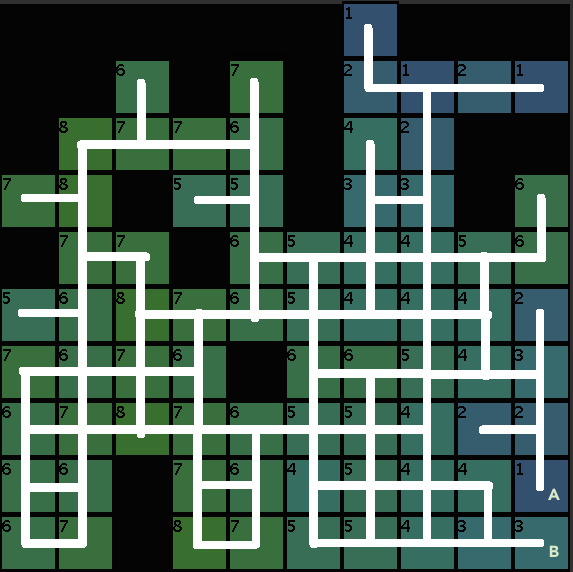
\includegraphics[width=.6\linewidth]{figures/connections}
	\caption{A battlefield, considered as a connected graph. The distance between points A and B at the bottom-right, despite the two points looking seemingly adjacent, is actually 9.}
	\label{fig:connected}
\end{figure}


The legal cells that a unit can move to are determined by the attribute \textit{move range}, which is a small positive integer. If we consider the battlefield as a connected graph with cells as vertices (figure \ref{fig:connected}), then given the move range $n$ the legal cells are all vertices whose shortest path from the current cell is at most $n$ cells away.

\subsection{Excluded elements}

There are some common characteristics of TRPG that are left out of this prototype.

\begin{itemize}

\item Experience system. Characters in RPG usually gain higher attributes or new skills from \textit{experience}. An experience system works by giving characters experience points from accomplishments, such as winning battles or completing quests. The points can then be converted into new abilities or increasing attribute values.

\item Equipment change within the battle, as another type of action in addition to attack and magic.

\item Items usage can also be added as another type of action.

\end{itemize}

 These are all common RPG traits. Including them, however, would elevate the level of complexity of the prototype, requiring much more efforts, especially on the competency of the AI. Leaving them out seems like a better option at this stage.

\section{Battle system}
\label{sub:battlesystemdesign}

We use the term `battle system' to refer to configurable parts of the battle model, which can be fine-tuned in order to bring desirable properties to the model. In this case, the objective, which will be expanded on further in section \ref{sub:battleobjectives}, is primarily to balance the role of jobs in the combat. We envision that this can be achieved by creating a set of parameters out of numerical values involved in various calculations in the battle. 

\subsection{Derived attributes calculation}

A large part of these parameters are for calculating derived attributes, which are functions of basic attributes.\footnote{The full list of derived attributes is given in appendix \ref{app:attributes}.} Preliminary design for these functions are as follows. First we consider the case of single-basic-attribute functions:
\begin{enumerate}
	\item As a preparation step, scale the value of the basic attribute into a number in the range $[0, 1]$, using the formula:
	\[
	scale(x) = \frac{x - min}{max - min}
	\]
	where $max$ and $min$ indicate the maximum and minimum possible values of the attribute's domain.
	\item At this stage we have transformed the basic attribute into a partial function defined in the domain $[0, 1]$, that grows linearly. This means units with higher attribute value would have an advantage over units with lower value in a uniform way. For example, if there are three units A, B, and C with scaled attribute value of 0.8, 0.6, and 0.4, respectively, then the amount of advantage of A over B would be the same as that of B over C, since $0.8 - 0.6 = 0.6-0.4$. We conjecture that it makes more sense to model this in a less restrictive way, allowing the advantage a variety of different \textit{shapes}.
	
	To accomplish this, the scaled attribute value from the previous step will be passed through a \textit{shaping function} $s(x)$, which maps the domain $[0, 1]$ onto itself. The function should be \textit{surjective} and \textit{monotonically increasing}, meaning that $s(0) = 0$, $ s(1) = 1$, and $x_1 \leq x_2 \implies s(x_1) \leq s(x_2)$. $x^2$ and $\sqrt{x}$ are examples of shaping functions that satisfied all these conditions.
	
	\item The last step is to reverse the scaling from the first step, mapping the result of the shaping function onto a final, target range $[min, max]$.
\end{enumerate}

As for the case of two input parameters, an extra step is needed between steps 1 and 2. After scaling both values to the appropriate range, they will be collapsed together into a single value using a bivariate function $f(x_1, x_2)$, such that the co-domain is still $[0, 1]$. One such function is the weighted average $\alpha x_1 + (1-\alpha) x_2$, where $\alpha$ is the weight given to the first parameter.

These functions will have to be implemented in such a way that its shape and range are highly configurable. The exact details are left to the implementation.

\subsection{Damage calculation}
\label{sub:dmgcalc}

Calculating damage is a complicated process that takes many inputs from the units and equipment involved. The calculation is slightly different between physical and magical attacks, but the principle is the same: first calculate the attacking potential of the attacker and defensive potential of the target, then use a similar formula to arrive at a single damage value. The result is modified further by a random variation.

The exact process is as follows. Let $X$ be the attacker, $Y$ be the target, $W$ be the attacking weapon, and $A$ be the armour worn by $Y$.

\begin{itemize}
	\item Calculate the \textit{attack power} ($ATK$). For physical attack, this is:
	
	\begin{center}
		$ATK$ = $X$'s physical attack potential $\times$ $W$'s physical attack power $\times$ $W$'s type physical coefficient
	\end{center}
	
	For magical attack, the level of the spell used is added to the calculation:
	
	\begin{center}
		$ATK$ = $X$'s magical attack potential $\times$ ($W$'s magical attack power + spell level bonus)
	\end{center}
	
	There are 3 levels of spells, and their bonus values, from level 1 to level 3, are \textit{fixed} to 0, 0.5, and 1. 
	
	\item Calculate the \textit{defensive power} ($DEF$) as the product of $Y$'s defensive potential, $A$'s defensive power, and the defensive coefficient -- a function of the attack type (melee, ranged, or magical) and the armour type.
	
	\item Calculate the \textit{base damage} ($DMG_0$) as $ATK \times \frac{ATK}{ATK+DEF}$. Notice that the last part of the multiplication is a value between 0 (when $DEF \gg ATK$) and 1 (when $ATK \gg DEF$), serving as a discount factor.
	
	\item In case of magical attack, base damage are multiplied by \textit{elemental advantage}, which is defined based on a coefficient $C_{elem}$. The value of this is either $C_{elem}$, $\frac{1}{C_{elem}}$, or $1$, depending on whether the element of the attacking magic and defending armour is at an advantage, disadvantage, or neutral, respectively.
	
	\item The actual damage $DMG$ is derived from the base damage and a random value $0 \leq r \leq 1$, as follows:
	\begin{center}
		$DMG = DMG_0 \times (r + 0.5)$
	\end{center}
	
	This means the actual damage can be anywhere in the range of 50\% to 150\% of the base damage.
\end{itemize}

The process includes a number of parameters, namely $C_{elem}$, the physical coefficient for the weapons (4), and the defensive coefficients for each pair of attack/armour types (9) -- a total of 14 parameters. 

\bigskip

Even with all these parameters, the whole battle progression could still be rather static, and a set of values that meets the intended objective to a satisfied degree might not exist. The implementation is free to make generalisation, adding more parameters as situations demanded.

\section{Battle controller}
\label{sub:battlecontroller}

The controller acts as a bridge between the players, the user interface, and the battle model. Its work can be described by the following pseudocode:

\begin{lstlisting}
initialize the battle model
while (battle has not ended):
  get next unit
  get the player controlling the unit
  get all valid moves
  while (unit has valid moves):
    ask the player to select one move
    update the battle model according to the move
    notify the UI to reflect changes in battle model
    recalculate valid moves
notify the UI that battle has ended
\end{lstlisting}

The communication between the controller and the user interface should be \textit{event-driven} e.g. implemented using design patterns such as \textit{observer} or \textit{publish-subscribe}. Event-driven programming is common in the MVC-style user interface, and another reason to prefer it is that other components than the UI might be interested in the progress of the battle as well -- one example is the battle system evaluator (section \ref{sub:battleeval}). Using event-driven paradigm would make observing the system very flexible.

\section{User interface}

The battle must be playable by human players, through a user interface. While graphical user interface is not required, it is preferable to a command-line one, since the game will be played by human volunteers as part of the project evaluation.

Here the capabilities needed to be implemented are listed.
\begin{itemize}
	\item Players must be able to select the combat command, and only valid commands are available for selection.
	\item Players must be able to follow the progress of the battle in an obvious, easy-to-understand fashion. This means it should be clear which unit is currently making decisions, what actions are taken, and what are the consequences.
	\item To help players make decision in an informed way, there must be a way for players to see the units' details, including the derived statistics, equipment, jobs, and races.
	\item The UI must be able to handle all valid battle systems.
	\item Battles between human player and AI are the absolute necessity that the UI must be able to facilitate. Player vs player and AI vs AI are desirable (it will be helpful in the development phase), but not required.
\end{itemize}

\section{Battle system objectives and evaluation}

\subsection{The objectives}
\label{sub:battleobjectives}

The goal of this work is to create a battle system that is in balance. As balance can be interpreted in a lot of different ways, we chose one perspective of balance as the primary objective: the \textit{combat triangle}.

Also known as the \textit{tactical rock-paper-scissors}, the combat triangle is one of the most common forms of balancing in combats.\cite[87]{moore2011basics} As in the original rock-paper-scissors game, among multiple elements involved there is no single element that emerges as the strongest one that always win over everything else -- each element has its own strength and weakness. This encourages players to try and utilise different combination of their available resources, making the game more challenging. Applying to this prototype, we adopted the system used in the game \gameref{runescape}, where the three attacking-type jobs (warrior, ranger, mage) each holds an intrinsic advantage over one other job, as follows:\cite{wiki-runescapecombat}
\begin{itemize}
	\item Warriors are strong against rangers, but weak against mages.
	\item Rangers are strong against mages, but weak against warriors.
	\item Mages are strong against warriors, but weak against rangers.
\end{itemize}

\begin{figure}
	\centering
	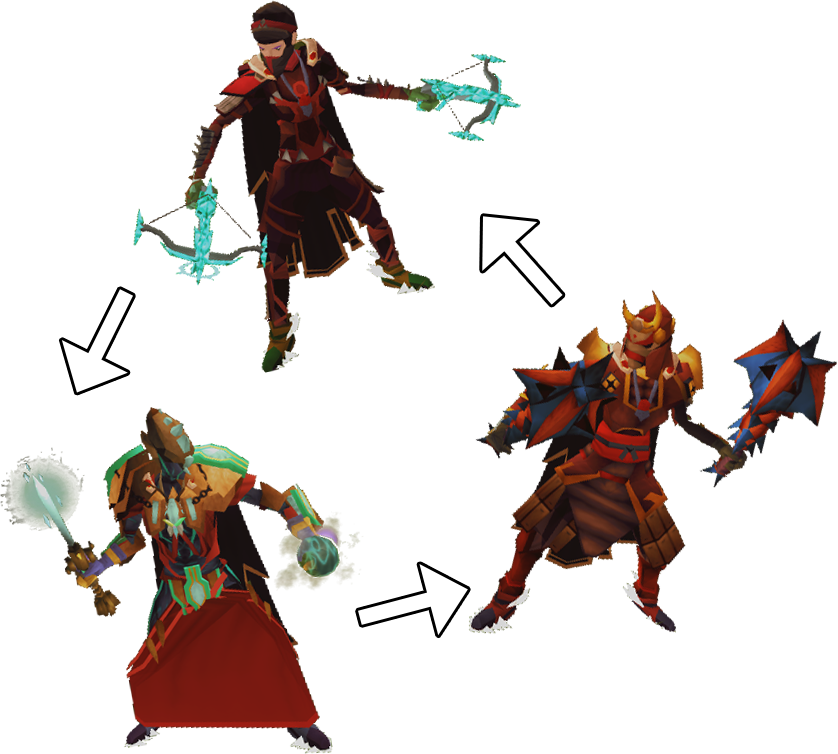
\includegraphics[width=.5\linewidth]{figures/runescape_triangle.png}
	\caption{The combat triangle for the game RuneScape.\cite{wiki-runescapecombat}}
\end{figure}

The other job, cleric, is not part of the combat triangle. As a supporting character class, we want it to have this following conflicting characteristics: (1) clerics should be weak attackers, but (2) the healing ability the job provides make parties with clerics stronger than those without. The contrast between individual weakness against group strength suggests that a balance is also required here. This is our secondary objective -- balancing the clerics against the other three attacking-type jobs.

Note that the three black magic elements -- fire, water, and nature -- also form their own tactical rock-paper-scissors. However to limit the level of complexity it will not be included as an objective.

\subsection{Battle system evaluation}
\label{sub:battleeval}

\subsubsection*{Evaluate a single constraint}

The method of evaluation depends on the objectives. For the combat triangle, we propose the following method of evaluation:
\begin{itemize}
\item Given two jobs, define a \textit{target win rate} as a number between 0 and 1. This is the target probability that the first job would win against the second on a random battle.
\item Simulate a number of random battles between the two jobs. First create two parties, one consists only of random units with the first job, and another with the second job. Then use the AI player to control the actions of both parties.
\item Count the number of times the first job wins the battle, and compare against the target win rate. The closer the actual win rate is to the target, the better.
\end{itemize}

The result of this method can be quantified by the \textit{objective function}, defined as the absolute difference between the actual win rate and the target win rate. The goal is then to minimise this function. We defined the target win rate as $0.8$ for all the advantages in the combat triangle.

As for the clerics-as-supporting-characters objective, the following targets are used:
\begin{itemize}

\item The win rate for a party with no clerics, against a party of clerics only, is set to 0.9 -- almost always. 
\item The win rate for a party with exactly one cleric, against a party with no clerics, is set to 0.7 -- a sizeable amount of advantage that is not too strong.
\end{itemize}

With a slight modification, the same evaluation method can also be used on this objective as well. Instead of specifying two jobs, two sets of \textit{job quotas} -- the exact number of units with the associated job -- are needed. All required constraints can be described in this way. For example, a party with exactly one cleric has a quota \texttt{[clerics = 1]}; an all-cleric party has quotas \texttt{[warriors = 0]}, \texttt{[rangers = 0]}, and \texttt{[mages = 0]}.

An implication of specifying objectives in this way is that the implementation would need to be able to support this kind of constraints upon instantiating battles.

\subsubsection*{Combining objectives}

If there is a single objective, then comparing battle systems is straightforward -- given our method of evaluation, the system that evaluate to the lowest value is the best. However there are already two major objectives -- the combat triangle and the clerics as helpful supporters. It is then not obvious how to compare these numerical values.

A sensible approach is to combined them into a single value. Researches in this area have offered a number of methods to achieve this task, as summarised in \cite{marler2004survey}. Some easy-to-implement options are min-max method, weighted sum, and weighted product. The optimisation process will need to experiment with these options to find out which gives the best result.

\section{The AI player}
\label{sub:aidesign}

The evaluation process we have laid out is based on the concept of \textit{self-play} -- simulating a number of battles using the same AI. The more competent the AI is, the better the evaluation.

The ultimate objective of the AI is to maximise its chance to win the battle. If the exact win probability is known for every possible instance of the battle, then the AI can simply choose the move that ends in the situation with the highest win probability. Unfortunately, that is not the case, as the exact win probability is difficult, if not impossible, to compute. Instead, we will use a heuristic based on the potential of each action to affect the amount of HP in the favourable direction to the AI's party.

Here we introduce the concept of \textit{HP-change potential}, which is a property of each possible action applied on a target unit. The actions are limited to the sensible ones: making damage to the enemies and healing units in the same party. The potential is defined as:
\[
	\Delta HP \times R^M
\]
where $\Delta HP$ is the expected change to HP (expected damage or expected recovery, as appropriate), $R$ is a discount coefficient between 0 and 1, and $M$ is the minimum number of moves required for the action taker to be able to execute the action.

The heuristic can be outlined as follows. First, the AI considers all its choices of action that can be done within this turn -- those which are immediately possible from the unit's current position, and those that are possible after moving the unit one time. It then finds the actions whose expected resulting effect would be largest, in terms of HP, i.e. the action with largest HP-change potential. If such an action exists, then:
\begin{itemize}
	\item If it can be executed immediately, then the AI would do it.
	\item If it requires a move, then the AI would move to one of the positions that allows it to make the action, then execute the action.
\end{itemize}

In the first case above, and in the case that no actions can be made, the unit would still have a free move that can be used to gain more advantage. In the second case, if there are multiple positions that allow the execution, then the AI should also choose the best among them. Choosing the best positions is done by considering the potential of each cell, from the following components:
\begin{itemize}
	\item $p_1$: the maximum HP-change potential the current unit can do from that position.
	\item $p_2$: The sum of all healing-type HP-change potential that all friendly units can do to the current unit, if it is in that position.
	\item $p_3$: The sum of all attacking-type HP-change potential that all enemy units can do to the current unit, if it is in that position.
\end{itemize}
The weighted sum $w_1 \cdot p_1 + w_2 \cdot p_2 - w_3 \cdot p_3$ is taken as the cell potential. All the weights should be configurable.

With this information, the `best move' is then easily defined, as the move to the cell with the highest cell potential.

\section{Battle system optimisation}

There are several optimisation techniques that might be applied to this task. One natural method that has been used in similar situations is \textit{genetic algorithm} (GA). GA is essentially a search-based technique. It systematically generates new solutions by maintaining a \textit{population} of possible solutions, which are initialised randomly, and try to create better solutions using the principle of natural selection, adopted from evolution in nature. The process prefers `fitter' members of the population -- those that give better evaluation result -- to survive and produce the next generation. Some of the weaker members also have some chance to survive in order to maintain variety in the population, as using only fitter members could quickly and easily leads to stagnation -- a local minimum. After a termination condition is fulfilled, the fittest member of the population is declared the best solution.

\section{Summary}

In this chapter the solution has been fully designed. The model and rules of the battle was laid out, and the configurable parts of the model was extracted out as the battle system. Basic requirements for the user interface was also described. We described how a reasonably competent AI player could be constructed, and how it would help in evaluating the battle system. Finally we proposed to use genetic algorithm as the strategy to arrive at a good battle system.